% !TEX encoding = UTF-8
% !TEX TS-program = pdflatex
% !TEX root = ../tesi.tex

%**************************************************************
\chapter{Performance}
\label{cap:performance}
%**************************************************************
\section{Confronto dei vari metodi}
In questa sezione confronteremo il tempo di esecuzione dei vari metodi risolutivi per 5 configurazioni iniziali del problema, di difficoltà crescente dal livello 0 al livello 4.\\
Per i primi 4 problemi abbiamo anche un dato del tempo impiegato da una persona nel risolvere il problema. Abbiamo infatti sottoposto i vari livelli a 8 persone diverse, di età compresa tra 16 e 55 anni, cronometrandoli durante lo svolgimento del gioco.\\
Per ogni livello sono presenti due tabelle: la prima contiene le misure di performance, in termini di tempo medio di esecuzione, rilevate per ogni tipo di solver; la seconda contiene invece il numero medio di stati attraversati da ogni solver per arrivare allo stato obiettivo. \\
Inoltre, per ogni tabella, si paragonano tra loro i risultati ottenuti da ogni solver con o senza le migliorie specificate in \ref{migliorie}
\subsection{Livello 0}
La configurazione iniziale del livello 0 è mostrata in figura \ref{lev0}. Le forme mancanti da inserire sono mostrate nelle figure \ref{z}, \ref{c}, \ref{y}.
\begin{figure}[h]
	\centering
	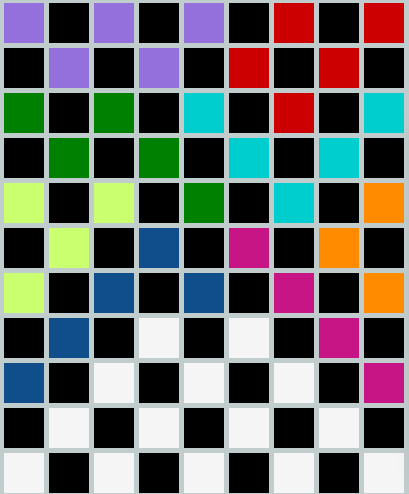
\includegraphics[scale=0.3]{immagini/lv0}
	\caption{Livello 0}
	\label{lev0}
\end{figure}
\\
\noindent


\begin{table} 
	\begin{tabular}{|l||*{4}{c|}}\hline 
		\backslashbox{Miglioria}{Solver} 
		&\makebox{DFS}&\makebox{Backtracking}&\makebox{Recursive Backtracking}	&\makebox{MinConflicts}\\ \hline 
		Sì&0.0192 (4.0)&0.0857 (11.0)&0.0708 (11.0)&0.0264 (1.0) \\ \hline 
		No&0.0786 (30.0)&0.0319 (11.0)&0.0327 (11.0)&0.0208 (1.0)  \\ \hline 
	\end{tabular} 
\end{table}
\begin{table} 
	\begin{tabular}{|l||*{4}{c|}}\hline 
		\backslashbox{Miglioria}{Solver} 
		&\makebox{DFS}&\makebox{Backtracking}&\makebox{Recursive Backtracking}	&\makebox{MinConflicts}\\ \hline 
		Sì&0.0483 (9.66666)&0.1135 (12.0)&0.1104 (12.0)&0.0668 (1.0) \\ \hline 
		No&0.2974 (147.5)&0.0480 (12.0)&0.0506 (13.0)&0.0910 (1.0)  \\ \hline 
	\end{tabular} 
\end{table}
\begin{table} 
	\begin{tabular}{|l||*{4}{c|}}\hline 
		\backslashbox{Miglioria}{Solver} 
		&\makebox{DFS}&\makebox{Backtracking}&\makebox{Recursive Backtracking}	&\makebox{MinConflicts}\\ \hline 
		Sì&0.3546 (78.3333)&0.1969 (22.0)&0.1874 (17.0)&0.3349 (1.0) \\ \hline 
		No&1.8782 (1472.5)&0.1241 (32.0)&0.0984 (19.0)&0.2641 (1.0)  \\ \hline 
	\end{tabular} 
\end{table}
\begin{table} 
	\begin{tabular}{|l||*{4}{c|}}\hline 
		\backslashbox{Miglioria}{Solver} 
		&\makebox{DFS}&\makebox{Backtracking}&\makebox{Recursive Backtracking}	&\makebox{MinConflicts}\\ \hline 
		Sì&36.227 (12343.8)&1.5018 (198.0)&0.5316 (55.0)&40.468 (15.1666) \\ \hline 
		No& ()&1.3156 (1179.0)&0.8229 (572.0)& ()  \\ \hline 
	\end{tabular} 
\end{table}
\begin{table} 
	\begin{tabular}{|l||*{4}{c|}}\hline 
		\backslashbox{Miglioria}{Solver} 
		&\makebox{DFS}&\makebox{Backtracking}&\makebox{Recursive Backtracking}	&\makebox{MinConflicts}\\ \hline 
		Sì& ()&1.4544 (184.0)&16.338 (2640.0)&24.502 (5.42857) \\ \hline 
		No& ()&5.1879 (4002.0)&26.403 (23971.0)& ()  \\ \hline 
	\end{tabular} 
\end{table}

\subsection{Livello 2}
La configurazione iniziale del livello 2 è mostrata in figura \ref{lev2}. Le forme mancanti da inserire sono mostrate nelle figure \ref{p}, \ref{smallv}, \ref{bigz}, \ref{i}, \ref{w}, \ref{v}.
\begin{figure}[h]
	\centering
	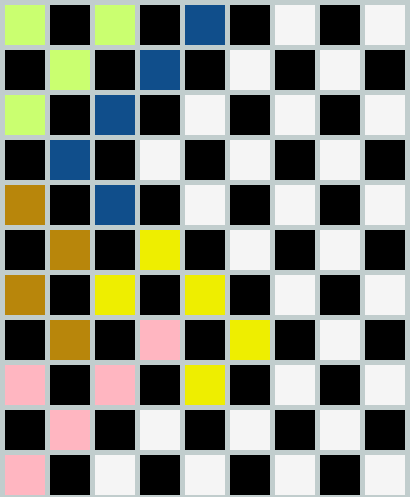
\includegraphics[scale=0.3]{immagini/lv2}
	\caption{Livello 2}
	\label{lev2}
\end{figure}

\subsection{Livello 3}
La configurazione iniziale del livello 3 è mostrata in figura \ref{lev3}. Le forme mancanti da inserire sono mostrate nelle figure \ref{z}, \ref{smallv}, \ref{bigz}, \ref{c}, \ref{y}, \ref{t}, \ref{w}, \ref{v}.
\begin{figure}[h]
	\centering
	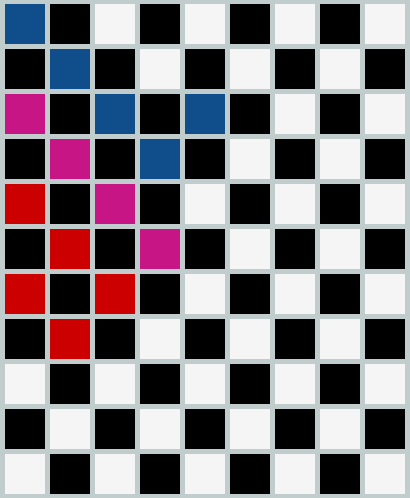
\includegraphics[scale=0.3]{immagini/lv3}
	\caption{Livello 3}
	\label{lev3}
\end{figure}

\subsection{Livello 4}
La configurazione iniziale del livello 4 è mostrata in figura \ref{lev4}. Tutte le forme devono essere inserite nella griglia.
\begin{figure}[h]
	\centering
	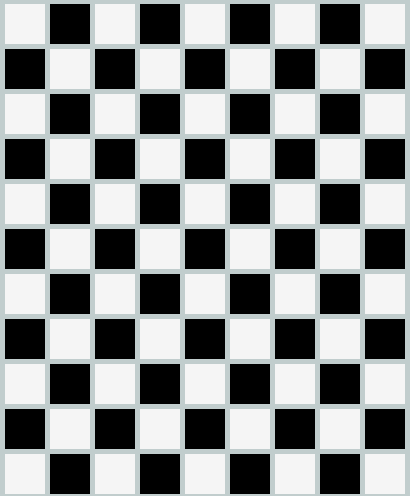
\includegraphics[scale=0.3]{immagini/lv4}
	\caption{Livello 4}
	\label{lev4}
\end{figure}


\section{Possibili miglioramenti}